% !TeX root = ../main-german.tex
\chapter{Hyperelliptische Kurven}

\section{Algebraische Varietäten und Geschlecht einer Kurve}
Für die Untersuchung hyperelliptische Kurven werden zunächst einige Grundlagen aus der algebraischen Geometrie eingeführt.

\begin{definition}[Affiner Raum]
  Der $n$-dimensionale affine Raum über einem Körper $K$ ist definiert als
  \[
    \mathbb{A}_K^n=\{(a_1,\dots,a_n)\mid a_i\in K\}.
  \]
\end{definition}
\cite[S.38]{Clader25}
Bestimmte Teilmengen des affinen Raumes lassen sich als gemeinsame Nullstellenmengen von Polynomen beschreiben. Diese werden als algebraische Mengen bezeichnet. Diese ist wichtig, da der affine Teil einer hyperelliptische Kurve durch die Nullstellenmenge ihrer Polynomgleichung dargestellt werden kann.
\begin{definition}
  Eine Teilmenge $Y\subset \mathbb{A}^n$ heißt eine algebraische Menge in $\mathbb{A}^n$, falls es eine Teilmenge $T\subset K[x_1,\dots,x_n]$ des Polynomrings gibt mit
  \[
    Y=\{P\in \mathbb{A}^n\mid f(P)=0 \text{ für alle }f \in T\}
  \]
\end{definition}
\cite[S.2--3]{Hulek12}
Aus der Algebra ist bekannt, dass ein Element $p$ irreduzibel beziehungsweise unzerlegbar ist, wenn $p$ nur triviale Teiler besitzt (vgl.~\cite[S.245--246]{Karpf24}). Eine algebraische Teilmenge $X$ hingegen heißt irreduzibel, wenn sie nicht als Vereinigung zweier echter algebraischer Teilmengen dargestellt werden kann. Wenn es also keine Zerlegung
\[
  X=X_1\cup X_2,\quad X_1,X_2\subsetneq X.
\]
in echte algebraische Teilmenge $X_1$ und $X_2$ exestiert. Alternativ wird $X$ reduzibel gennant.
\cite[S.18]{Hulek12}
\begin{definition}[Affine Varietäten]
  Sei $K$ ein Körper. Eine Menge $X\subseteq\mathbb{A}^n$ heißt eine affine algebraische Varietät, wenn $X$ irreduzibel ist.
\end{definition}
\cite[S.39,43]{Clader25}
Doch die affine Ebene kann nicht alle Punkte beschreiben, denn es fehlen sonst die Punkte im Unendlichen. Um daher ein besseres Verhalten für die Varietäten zu erhalten, wird der projektive Raum benötigt.
\begin{definition}[Projektive Ebene]
  Sei $K$ ein Körper. Die projektive Ebene über $K$ ist definiert als
  \[
    \mathbb{P}^2_K
    =
    \left(K^3 \setminus \{(0,0,0)\}\right)/\sim,
  \]
  wobei für
  \[
    (X,Y,Z),(X',Y',Z') \in K^3 \setminus \{(0,0,0)\}
  \]
  die Äquivalenzrelation \((X,Y,Z)\sim(X',Y',Z')\) genau dann gilt, wenn ein $\lambda \in K^\times$ existiert mit \((X,Y,Z)=\lambda(X',Y',Z')\).
  Die Äquivalenzklasse eines Tripels $(X,Y,Z)$ wird mit \([X:Y:Z]\) bezeichnet und heißt Punkt der projektiven Ebene.
\end{definition}
\cite[S. 245--246]{Clader25}
\begin{definition}[Projektvie Varietät]
  Eine porjektive Varietät ist eine Teilmenge $V\subset \mathbb{P}_K^n$, sodass es eine Menge homogener Polynome $T\subset K[x_0,\dots,x_1]$ exestiert, sodass
  \[
    V=\{P\in\mathbb{P}_K^n\mid f(P)=0 \text{ für alle } f\in T\}
  \]
  und die Menge $V$ irreduzibel ist.
\end{definition}
\cite[S.55]{Hulek12}

Genauso wie bei Kurven sollen nun auch bei Varietäten singuläre Punkte definiert werden.
\begin{definition}
  Ein Punkt $P$ auf einer Varietät $V$ heißt singulär, wenn es ein $i$ gibt mit \(\frac{dx}{dx_i}(P)=0\). Ansonsten heißt $P$ glatter, regulärer oder nichtsingulärer Punkt der Varietät $V$.
\end{definition}
Der Grad eines Polynoms einer Kurve kann als Grad der Kurve bezeichnet werden. (Noch Quelle einfügen)
one-dimensional projective varieties—otherwise
known as algebraic curves \cite[S.409]{Clader25}
Ein topologischer Raum ist eine Menge $X$, welche mit einer Topologie versehen wird, die festlegt welche Teilmenge von $X$ als offen gilt.
\begin{definition}[Dimension]
  Sei $X$ ein topologischer Raum. Die Dimension von $X$ ist definiert als
  \[
    \dim(X)=\sup\left\{
    n\in\mathbb{N}_0 \;\middle|\;
    Z_0\subsetneq Z_1\subsetneq\cdots
    \subsetneq Z_n\subseteq X
    \right\},
  \]
  wobei $Z_i$ distinkt verschieden, irreduzible und abgeschlossene Teilmenge von $X$ sind. Die Dimension einer affinen oder projektiven Varietät ist genau gleich der Dimension des topologiscehn Raums.
\end{definition}
Wenn man $\mathbb{A}^1$ betrachtet, sind die einzigen Untermengen von $\mathbb{A}^1$ der gesamte Raum oder ein einzelner Punkt. Daraus folgt \(\dim(\mathbb A_K^1)=1\).
\cite[S.5--6, 10]{Hartshorne7}

\begin{definition}[Algebraische Kurve]
  Eine algebraische Kurve ist eine algebraische Varietät der Dimension $1$.
\end{definition}
\cite[S.137]{Hulek12}

\begin{remark}
  Im Folgenden werden ausschließlich glatte projektive algebraische Kurven betrachtet. Ein glatte Kurve ist hierbei eine Kurve, die in mindestens einer der beiden partiellen Ableitungen ungleich null ist.
\end{remark}
\cite{S.82}{Hulek12} und Clader eventuell noch


\begin{definition}[Geschlecht einer Kurve]
  In der Topologie bezeichnet es die meisten Schnitte, sodass das Objekt noch verbunden ist.
  In der algebraischen Geometrie: Geometrischer Genus \(g=\frac{(d-1)(d-2)}{2}-s\), wobei $s$ die Anzahl der Singularitäten ist.
\end{definition}
Ein Tourus hat daher Geschlecht 1 und ein Torus mit 2 Löchern Geschlecht 2.
\section{Hyperelliptische Kurven}

\subsection{Grundlagen der hyperelliptischen Kurven}
Hyperelliptische Kurven sind eine spezielle Klasse algebraischer Kurven und können daher als eine Generalisierung von elliptischen Kurven betrachtet werden. Eine elliptische Kurve besitzt das Geschlecht $g=1$, wohingegen hyperelliptische Kurven auch ein höheres Geschlecht haben können.

\cite[2--4]{Menezes96}
\cite[S.304]{Cohen06},\cite[407--408]{Washington08}
\begin{definition}
  Sei $K$ ein Körper mit dem algebraischem Abschluss $\overline{K}$ und $g\geq 1$. Eine hyperellitpische Kurve $C$ vom Geschlecht $g$ über $K$ ist durch die Gleichung
  \[
    C:\quad y^2+h(x)y=f(x)
  \]
  mit $h,f\in K[x]$, $\deg(h)\leq g$  und $\deg(f)=2g+1$, wobei $f$ normiert ist, definiert. Gleichzeitig wird wie bei elliptischen Kurven vorrausgesetzt, dass die Kurve keine singulären Punkte besitzt, also dass es keine Punkte $P=(x,y)\in\overline{K}$ gibt mit
  \begin{align*}
    y^2+h(x)y=f(x)                                    \\
    2y+h(x)=0 \quad \text{paritelle Ableitung nach y} \\
    h'(x)y-f'(x)=0 \quad \text{partielle Ableitung nach x}
  \end{align*}
  Außerdem besitzt die Kurve genausow ie eine elliptische Kurve einen Punkte mit Unendlich bezeichnet mit $\infty$.
\end{definition}
Das negative von $P=(x,y)$ ist gegeben durch $-P=(x,-y-h(x))$.

\begin{remark}
  Eine elliptische Kurve ist nach diesen Bedingungen eine Kurve mit dem Geschlecht $1$. Daher sind auch die algorithmischen Eigenschaften die gleichen.
\end{remark}

\begin{example}
  Sei $E$ mit $y^2=x^5+1184x^3+1846x^2+956x+560$ eine hyperelliptische Kurve des Geschlechtes $2$. Diese Bedingung soll nun überprüft werden.
  Es gilt $2y$ ist $0$, genau dann wenn $y=0$ ist. Dadurch erhält man einen Punkt $P=(x_1,0)$, genau dann wenn $f(x_1)=0$ ist. Für die partielle Ableitung von $x$ gilt, $f'(x)=5x^4+1549x^2+1689x+956$. Es erfüllt keine Wurzel von $f$ gleichzeitig $f'$ erfüllt.

  Allgemein $f'$ wird $0$ als Wurzel von $x_1$ von $f$, genau dann wenn $x_1$ ist eine vielfache Nullstelle von $f$. Für ungerade Charakteristik ist die Gleichung $y^2=f(x)$ eine nichtsinguläre und damit hyperelliptische Kurve, wenn $f$ keine mehrfachen Nullsten besitzt.
\end{example}





\cite[S.3]{Menezes96}
\begin{lemma}
  Sei $C$ eine hyperelliptische Kurve über $K$ wie in der Definition.
  \begin{enumerate}
    \item Wenn $h(u)=0$, dann ist $\operatorname{char}(K)\neq 2$
    \item Wenn $\operatorname{char}(K)\neq 2$, dann transformiert der Variablenwechsel $u\rightarrow u, v\rightarrow(v-h(u)/2)$ die Kurve $C$ zu der Form $v^2=f(u)$ mit $\deg_u(f)=2g+1$. (Diese Schreibweise einführen oder entfernen)
  \end{enumerate}
\end{lemma}
\begin{proof}
  In \cite[S.3--4]{Menezes96}
\end{proof}

Sei $L$ eine Körpererweiterung von $K$. Die Menge aller $L$-rationalen Punkte der Kurve $C$ besteht aus den affinen Punkten, deren
Koordinaten in $L$ liegen, sowie dem Punkt im Unedlcihen der mit $\mathcal{O}=\infty$ bezeichnet wird
\[
  C(L)=\{(x,y)\in L\times L\mid y^2+h(x)y=f(x)\}\cup\{\mathcal{O}\}.
\]
\begin{figure}[htbp]
  \centering
  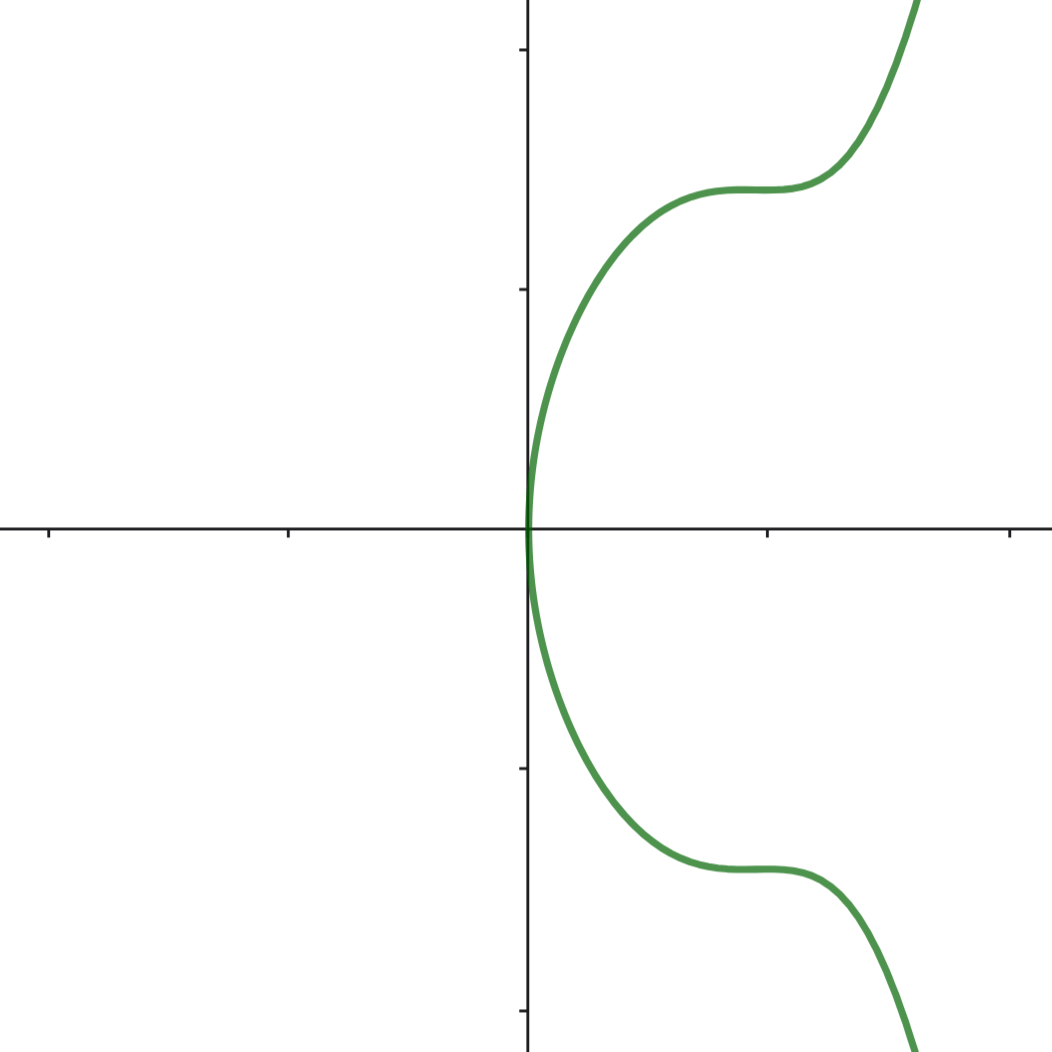
\includegraphics[width=0.4\textwidth]{images/hyp_elip_curve_1.png}
  \caption{Hyperelliptische Kurve mit $y^2=x^5-3x^3+4x$ über $\mathbb{R}$.\\
    {\footnotesize Quelle: Eigene Darstellung mit GeoGebra}}
\end{figure}
\begin{figure}[htbp]
  \centering
  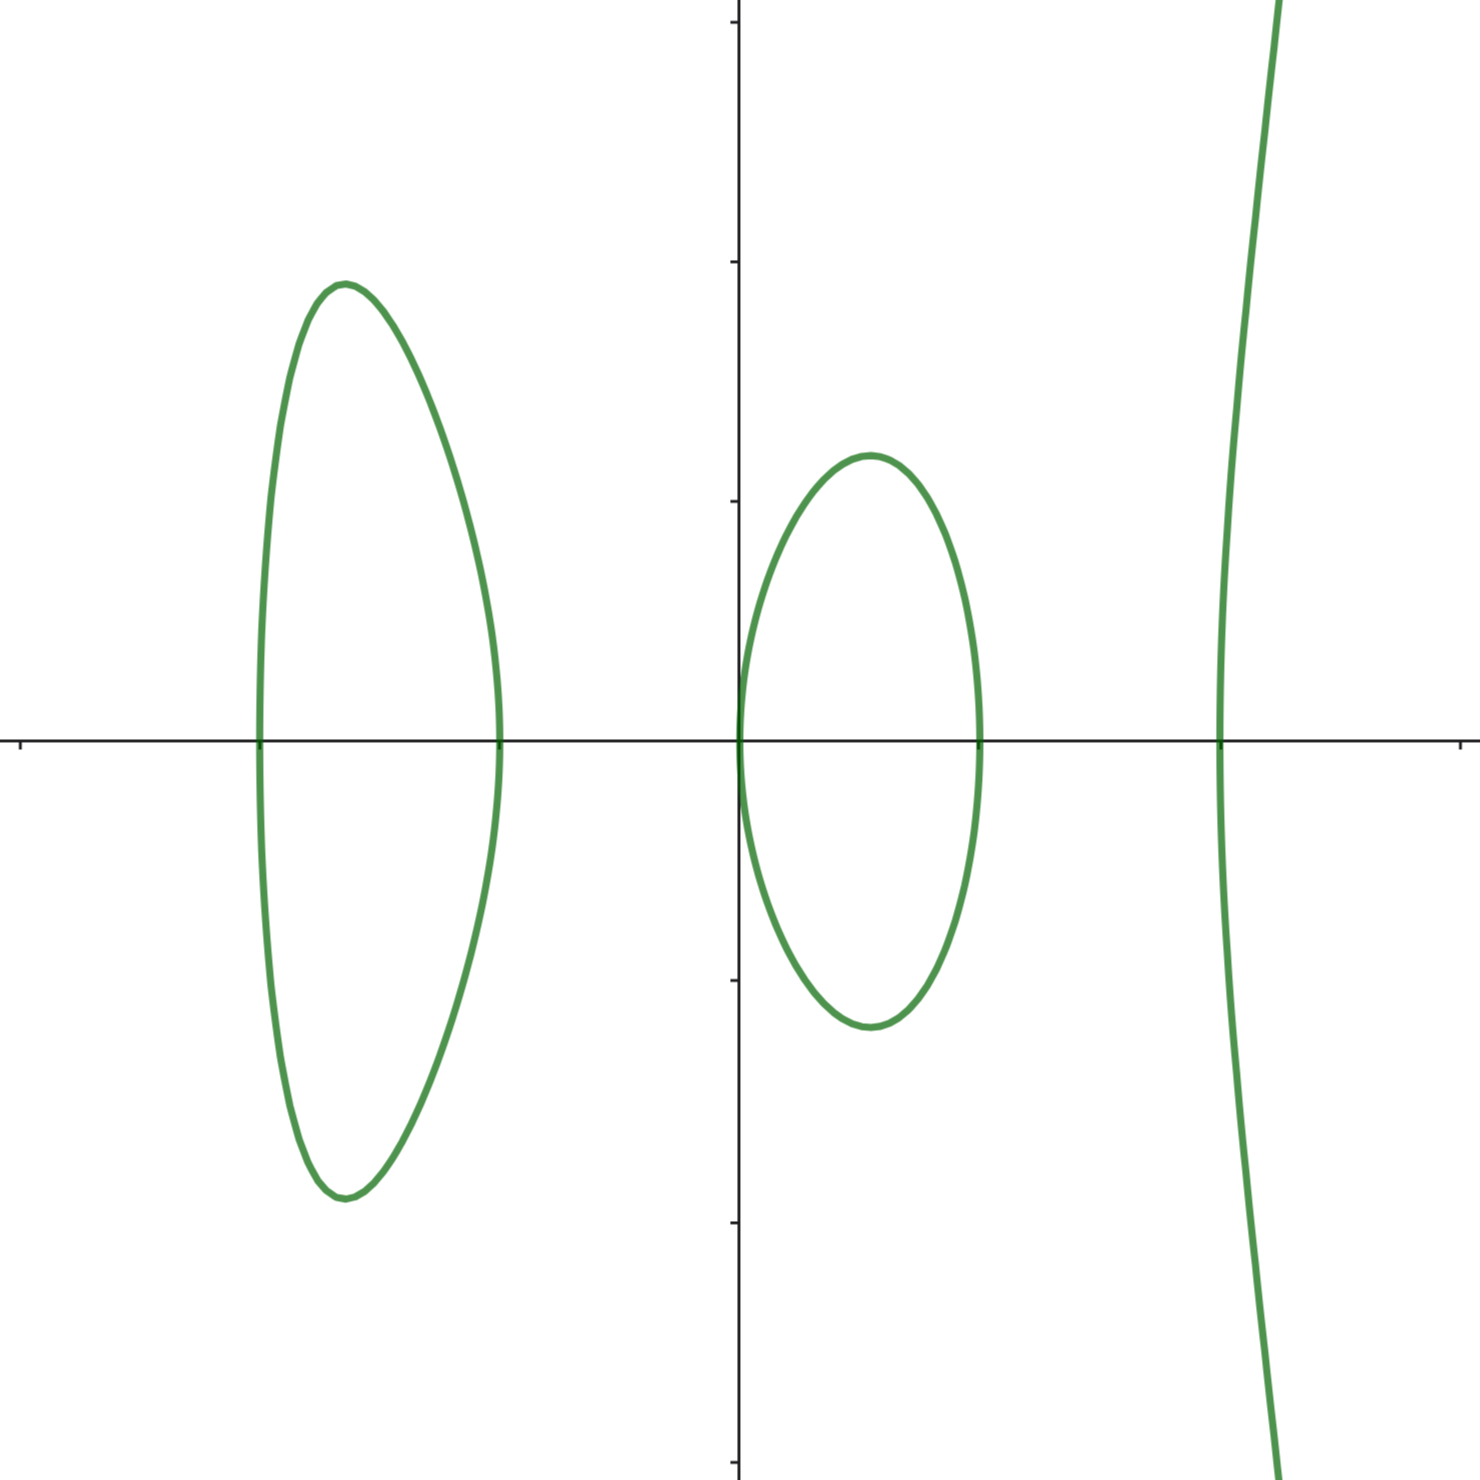
\includegraphics[width=0.4\textwidth]{images/hyp_elip_curve_2.png}
  \caption{Hyperelliptische Kurve mit $y^2=x^5-5x^3+4x$ über $\mathbb{R}$.\\
    {\footnotesize Quelle: Eigene Darstellung mit GeoGebra}}
\end{figure}

\begin{example}
  Es ist auch möglich hyperellitpische Kurven über endlichen Körper zu formulieren. Sei $C:y^2=x^5+x+1$ eine hyperelliptische Kurve über dem Körper $\mathbb{Z}_{11}$. Es ist hierbei $h(x)=0$, $f(x)=x^5+x+1$
\end{example}
\begin{definition}[Ordnung von einer Polynomfunktion in einem Punkt]\label{def:ord-punkt}
  Sei $G=a(x)-b(x)y\in \overline{K}[C]$ und $P\in C$. Die Ordnung von $G$ im Punkt $P$ wird durch $\operatorname{ord}_P(G)$ geschrieben und ist wie folgt definiert
  \begin{enumerate}
    \item Wenn $P=(x',y')$ ein endlicher Punkt ist, dann sei $r$ der größte Exponent von $(x-x')$ der sowohl $a(x)$ als auch $b(x)$ dividiert. Es kann dann geschreiben werden $G(x,y)=(x-x')^r (a_0(x)-b_0(x)y)$. Wenn nun $a_0(x')-b_0(x')y*\neq 0$, dann ist $s=0$, ansonsten ist $s$ der größte Exponent von $(x-x')$ der $N(a_0(x)-b_0(x)y)=a_0^2+a_0b_0h-b_0^2f$ teilt. Wenn $P$ ein ordinärer Punkt ist, dann ist $\operatorname{ord}_P(G)=r+s$. Wenn es ein spezieller Punkt ist, dann ist $\operatorname{ord}_P(G)=2r+s$.
    \item Wenn $P=\infty$ dann gilt
          \[
            \operatorname{ord}_P(G)=-\max(2\deg_u(a),2g+1+2\deg_u(b)).
          \]
  \end{enumerate}
\end{definition}

\subsection{Divisoren}
\begin{definition}
  Der Funktionenkörper von V ist der Quotientenkörper $k(V)=\operatorname{Quot}(k[V])$. Die Elemente $f\in K(V)$ heißen rationale Funktionen auf $V$.
\end{definition}
\begin{definition}[Ordnung einer Polynomfunkton an einem Punkt]
  Sei $G=a(u)-b(u)v\in \overline{K}[C]$ und $P\in C$. Dann ist die Ordnung von $G$ in $P$ definiert durch $\operatorname{ord}_P(G)$ mit
  \begin{enumerate}
    \item Wenn $P=(x,y)$ endlich ist, dann ist die Ordnung der führende Koeffizient von $G$.
    \item Wenn $P=\infty$ dann ist $\operatorname{ord}_P(G)=-\max(2\deg_u(a),2g+1+2\deg_u(b))$.
  \end{enumerate}
  \textbf{Noch sinnvoll definieren}
\end{definition}
\cite[S.14]{Menezes96}
Keeping track of the number of zeros and poles of a function or differential
suggests the concept of divisor, which on a compact Riemann surface is
simply a formal sum of points-with-multiplicity.
\begin{definition}[Divisor]
  Ein Divisor $D$ auf $C$ ist eine endliche Summe
  \[
    D=\sum_{P\in C}m_P P, \quad m_P\in\mathbb{Z}
  \]
  Der Grad ist definiert durch
  \[
    \deg D = \sum_{P\in C}^{m_P}
  \]
  Die Ordnung ist definiert durch $operatorname(ord)_P(D)=m_P$
\end{definition}
\cite[S.16]{Menezes96}
\cite[S.137--]{Hulek12}
\begin{definition}[Divisorgruppe]
  Sei $C$ eine Kurve über dem Körper $K$. Dann ist die Divisiorgruppe $\operatorname{Div}_C$ von $C$ die freie (eventuell auch noch definieren) abelsche Gruppe, die von Punkten von $C$ erzeugt wird. Ein Element $D\in\operatorname{Div}_C$ wird ein Divisor genannt. Er ist gegeben durch
  \[
    \operatorname{Div}_C=\{D\mid D\text{ ist ein Divior auf }C\}
  \]
  Zusammen mit der Addition formt die Divisorengruppe eine Gruppe (noch zeigen)
  \[
    D_1+D_2= \sum_{P\in C}(n_P+m_P)P.
  \]
  Die Menge aller Divisoren vom Grad 0 wird mit $D^0$ bezeichnet und ist eine Untergruppe von $D$(eventuell auch zeigen).
\end{definition}
\begin{definition}[Hauptdivisior]
  Sei $C$ eine Kurve über dem Körper $K$. Ein Divisor $D\in\operatorname{Div}_C$ heißt Hauptdivisor, wenn eine rationale Funktion $f\in\overline{K}(C)^\times$ existiert, sodass
  \[
    \operatorname{div}= \sum_{P\in P}\operatorname{ord}_P(f)P.
  \]
  Wenn für die Funktion $f=g/h$ gilt dann ist $\operatorname{div}(f)=\operatorname{div}(h)-\operatorname{div}(h)$.
\end{definition}
\cite[S.67]{Cohen06}
\cite[S.140]{Hulek12}
Es wird die Gruppe aller Hauptdivisoren auf der Kurve $C$ mit $\operatorname{Princ}_C$ bezeichnet.
\begin{theorem}
  Sei $C$ eine projektive algebraische Kurve über einem algebraisch abgeschlossenen Körper $\overline{K}$ und $G\in\overline{K}(C)^\times$. Dann hat $G$ eine endliche Anzahl an Nullstellen und Polen. Außerdem gilt $\sum_{P\in C}\operatorname{ord}_P(G)=0$.
\end{theorem}
Für den Beweis werden noch ein paar mathematische Werkzeuge benötigt. Sei $G(x,y)=a(x)-b(x)y\in \overline{K}[C]$. Es gilt dann für die algebraische Norm $N(G)=G\overline{G}$ und den Grad $\deg(G)=\max(2\deg_x(a),2g+1+2\deg_x(b))$, die Eigenschaften dieser werden hierfür aus~\cite[S.~7--9]{Menezes96} herangezogen.
\begin{proof}
  Zunächst sei $G=a(x)-b(x)y\in \overline K[C]\setminus\{0\}$ eine Polynomfunktion.  Sei $n=\deg(G=\max\{2\deg_x(a),\,2g+1+2\deg_x(b)\})$. Für die algebraische Norm $N(G)=G \overline G$ gilt nach~\cite[S.~9, Lemma 16]{Menezes96} \(\deg_x(N(G))=\deg(G)=n\). Da $\overline{K}$ algebraisch abgeschlossen ist, kann die Norm als
  \[
    n(G)=G\overline{G}=(x-x_1)(x-x_2)\cdots(x-x_n), quad x_i\in \overline{K}.
  \]
  geschrieben werden. Jede Nullstelle $x_i$ hat auf der hyperelliptischen Kurve die
  Nullstellenordnung $2$. Daher gilt \( \sum_{P\neq\infty}\operatorname{ord}_P(N(G))=2n\). Es folgt dann mit $N(G)=G\overline{G}$ und der Additivität der Ordnung, dass
  \[
  2n=
  \sum_{P\neq\infty}\operatorname{ord}_P(G)
  +
  \sum_{P\neq\infty}\operatorname{ord}_P(\overline G).
  \]
  Wegen Anwenden Lemma~\cite[S~15, Lemma 28]{Menezes96} gilt \(\sum_{P\neq\infty}\operatorname{ord}_P(G)=\sum_{P\neq\infty}\operatorname{ord}_P(\overline G)\). Damit gilt dann
  \[
  \sum_{P\neq\infty}\operatorname{ord}_P(G)=n.
  \]
  Es gilt dann im Punkt am Unendlichen \(\operatorname{ord}_P(G)=-\deg(G)=-n\). Dann folgt insgesamt
  \begin{align*}
    \sum_{P\in C}\operatorname{ord}_P(G) &= \sum_{P\neq \infty}\operatorname{ord}_P(G)+\operatorname{ord}_P\infty(G)\\
    &= n-n\\
    &= 0.
  \end{align*}
\end{proof}
\cite[S.15]{Menezes96} und \cite[S.~97]{Fuelton08}
\begin{remark}
  Damit ist dann auch der Divisor einer rationalen Funktion $(f)$ eine formale Summe und es gilt $\deg(\operatorname{div}(f))=0$.
\end{remark}
\begin{example}
  Sei $C:y^2-5x^3+4x$ eine hyperelliptische Kurve und $f(x,y)=y$. Dann berechnet man die Schnittpunkte der Kurve $C$ mit $f$, dass ergibt die Schnittpunkte
  \[
    P_1=(-2,0),P_2=(-1,0),P_3=(0,0), P_4=(1,0), P_5=(2,0).
  \]
  Die Funktion $f$ besitzt an jedem Punkt eine Nullstelle erster Ordnung. Aufgrund der Definition der Kurve besitzt $f$ eine Polstelle fünfter Ordnung am Punkt im Unendlichen. Daher gilt
  \[
    \div(f)=(P_1)+(P_2)+(P_3)+(P_4)+(P_5)-5(\infty).
  \]
  \begin{figure}[htbp]
    \centering
    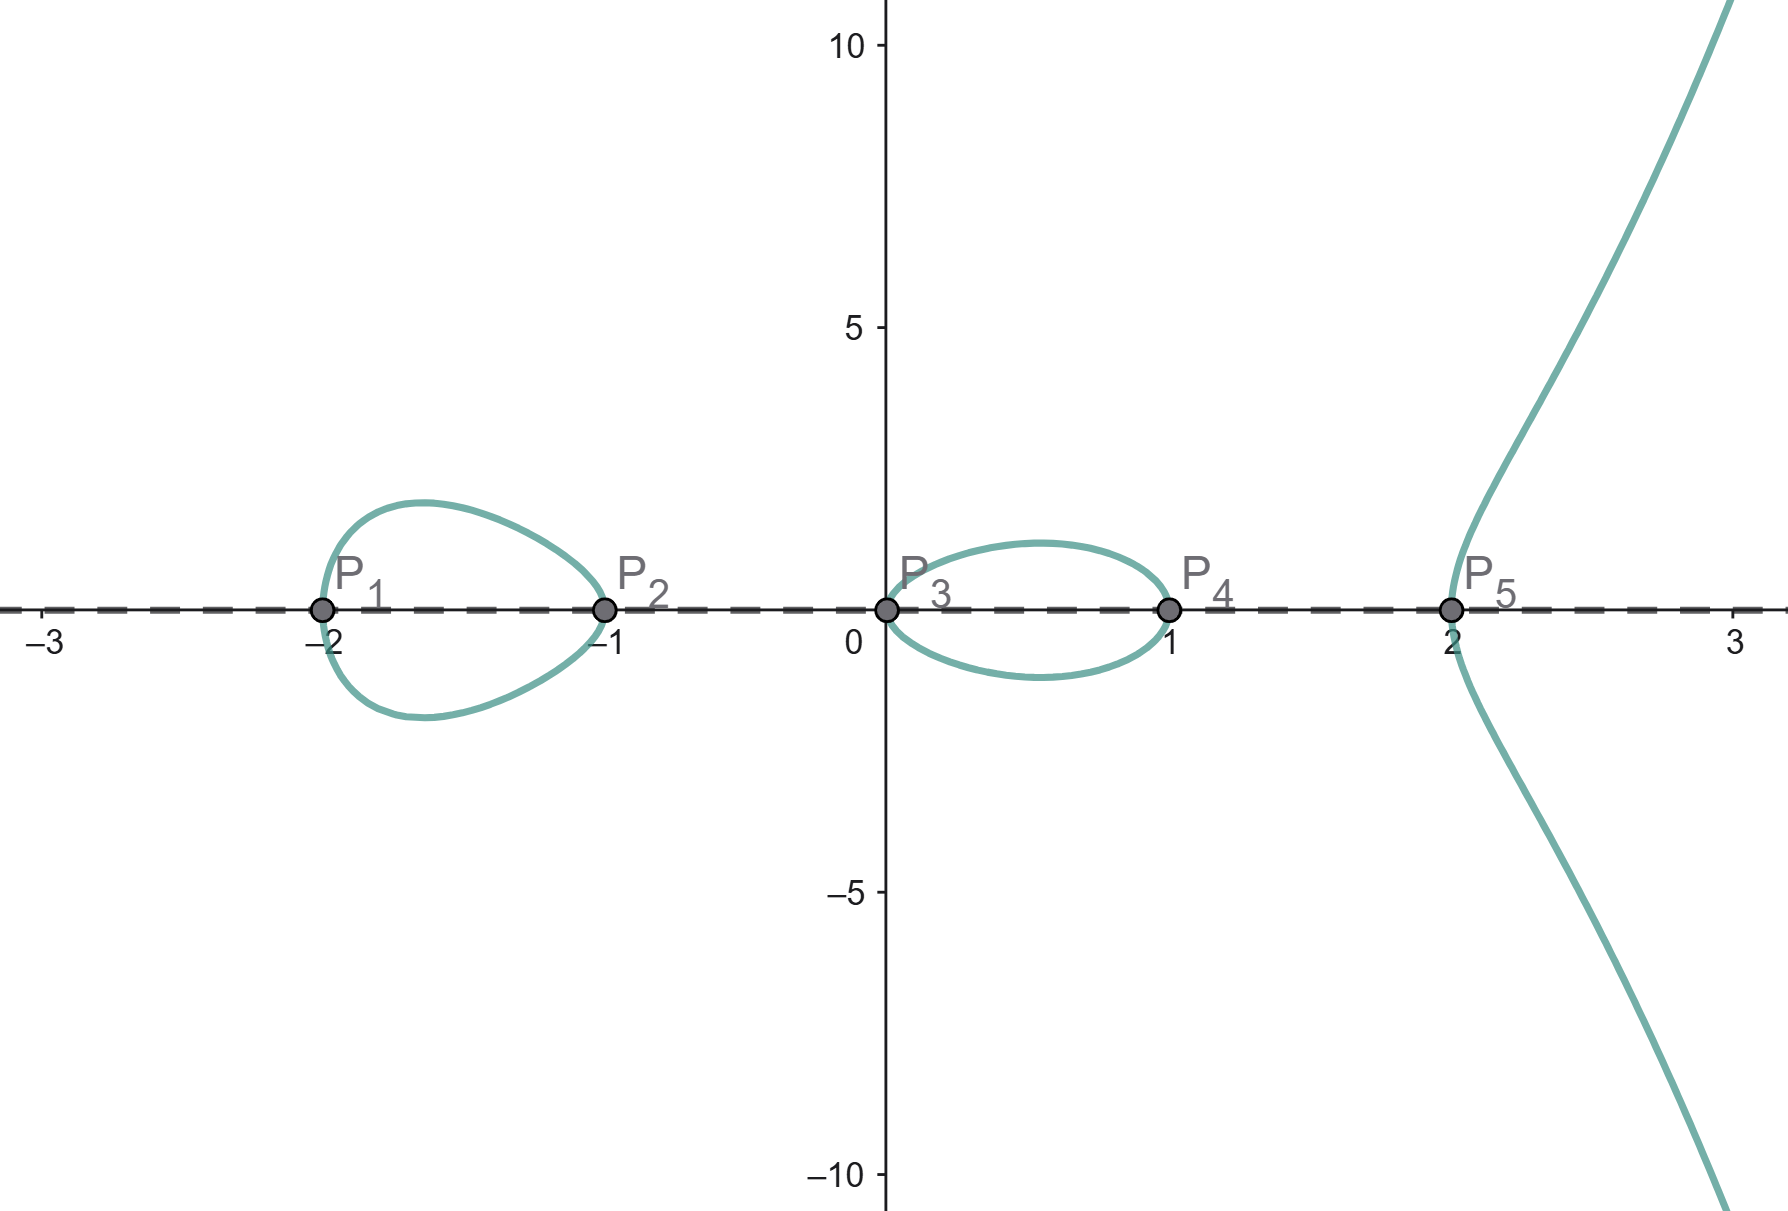
\includegraphics[width=0.4\textwidth]{images/hyp_hauptdivisor_1.png}
    \caption{Hyperelliptische Kurve mit $y^2=x^5-3x^3+4x$ über $\mathbb{R}$. Und Darstellung des Hauptdivisors.\\
      {\footnotesize Quelle: Eigene Darstellung mit GeoGebra}}
  \end{figure}
\end{example}
\begin{definition}[Divisorklassengruppe und Jacobische]
Sei $C$ eine glatte projektive Kurve. Dann ist die Divisorklassengruppe von $C$ definiert durch
  \[
  \operatorname{Cl}_C=\frac{\operatorname{Div}_C}{\operatorname{Princ}_C}.
  \]
  Die Jacobische von $C$ ist dann die Gruppe der Divisorklassen vom Grad null, also
  \[
  \operatorname{Jac}_C=\frac{\operatorname{Div}^0_C}{\operatorname{Princ}_C}.
  \]
  Seien nun $D_1,D_2\in \operatorname{Div}_C^0$ dann schreibt man für zwei linear Äquivalente Divisoren $D_1\equiv D_2$, wenn $D_1-D_2\in \operatorname{Pic}$ für ein $f\in K$
\end{definition}
\cite[S.17]{Menezes96}
Wie man sieht kann man mit $\operatorname{div}(f)$ die Schnittpunkte der Funktion $f$ und der Kurve $C$ zählen. Zwei Vektoren sind linear Äquivalente Divisoren, wenn $D'=D+\div(f)$ für ein $f\in K$. Dann schreibt man $D'\equiv D$. Im folgenden ist $D'$ der linear äquivalente Divisor zu $D$.

Es ist dann $\operatorname{div(v)}=(S)+(R)-2\infty$ die vertikale Line mit der Spiegelung.

$\operatorname{div}(l/v)=(P)+(Q)-(R)-(\infty)$


\begin{definition}
  Sei $C$ eine Kurve, dann ist ihre Divisorklassengruppe definiert durch
  \[
    \operatorname{Cl}(C) = \operatorname{Div}C/~.
  \]
\end{definition}
\begin{lemma}
  Die Hauptdivisoren bilden eine Untergruppe und daher ist die Divisorenklassengruppe $\operatorname{Cl}(C)$ eine abelsche Gruppe.
\end{lemma}
\begin{proof}
  Noch einfügen Aussage auch aus \cite[S.141]{Hulek12} hier aber kein lemma.
\end{proof}
\cite[S.141]{Hulek12}
Jeder Hauptdivisor hat den Grad 0. Erzeugt die Gradfuntion einen Homorphismus
\[
  \deg:Cl(C) \rightarrow \mathbb{Z}
\]
\cite[S.149]{Hulek12}


\subsection{Divisorklasse und reduzierte Divisoren}
Es soll nun gezeigt werden wie man analog wie bei elliptischen Kurven die Addition auf der Gruppe der hyperellitpischen Kurve berechnet. Sind das reduzierte Divisoren?
\begin{definition}[Reduzierter Divisior]
  Ein reduzierter Divisor ist $D=\sum m_iP_i-\sum m_i\infty$, wobei $m_i\geq 0$ und alle $P_i$ endliche Punkte sind, für die gilt $m_P\neq 0$ .mit $\sum m_i\leq g$ und dabei ist $g$ das Geschlecht von $C$
\end{definition}
\cite[S.17]{Menezes96}
Es soll nun betrachtet werden wie die Addition zweier Divisoren auf einer hyperelliptischen Kurven abläuft. Sei dafür $C:y^2=x^5-5x^3+4x+1$ auf dieser liegen die Punkte $P_1=(-2,0),P_2=(-1,0),P_3=(0,0), P_4=(1,0)$, durch diese werden die zwei Divisoren $D_1=(P_1)+(P_2)-2(\infty)$ und $D_2=(P_3)+(P_4)-2(\infty)$. Es kann dann die Summe aus beiden Divisoren gebildet werden $D=D_1+D_2=\sum_{i=1}^{4}(P_i)-4(\infty)$.

\begin{figure}[htbp]
  \centering
  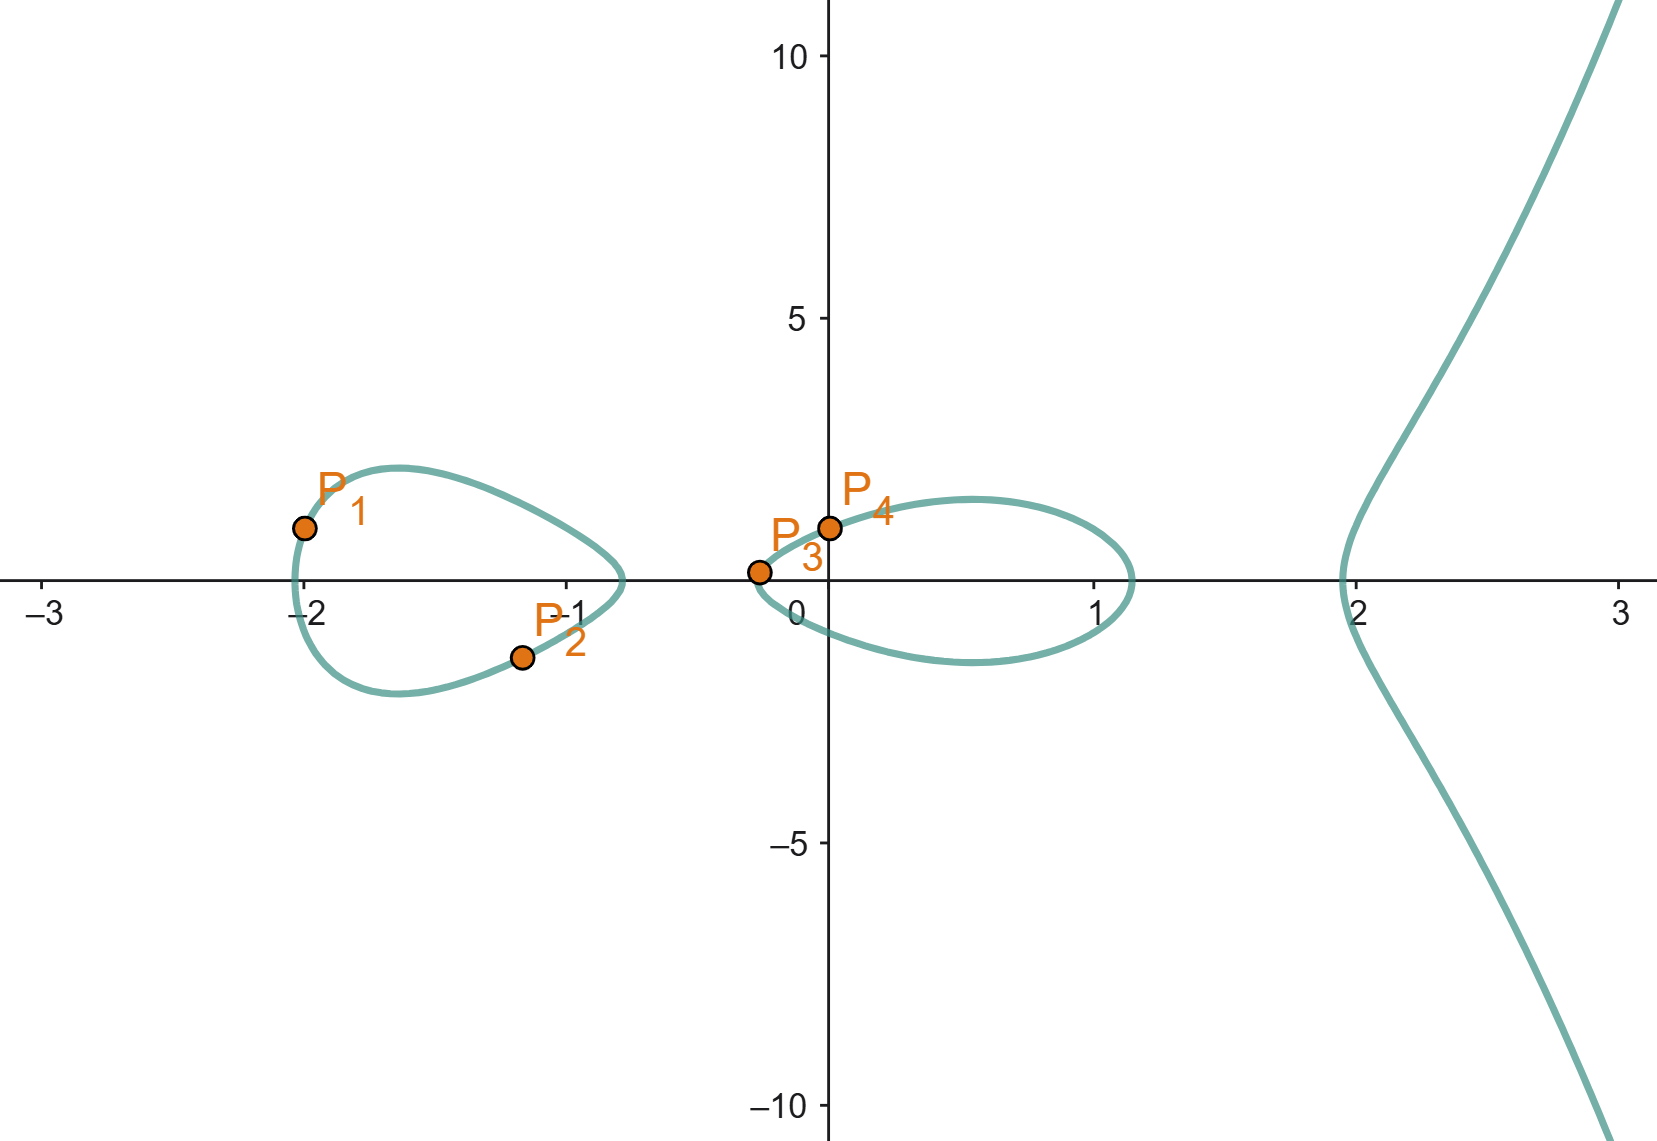
\includegraphics[width=0.4\textwidth]{images/div_add_1.png}
  \caption{Hyperelliptische Kurve mit $y^2=x^5-3x^3+4x+1$ über $\mathbb{R}$.\\
    {\footnotesize Quelle: Eigene Darstellung mit GeoGebra}}
\end{figure}
Durch diese vier Punkte wird ein kubisches Polynom gelegt, dass durch die Funktion $f(x,y)= -\frac{4}{5}x^3+\frac{16}{5}x+1$ beschrieben wird. Wenn man nun die linke Seite der Kurve $f(x)-f(x,y)^2=0$ rechnet, erhöt man eine Gleichung 6 Grades (hier Variable sinnvoll noch ändern).
\begin{figure}[htbp]
  \centering
  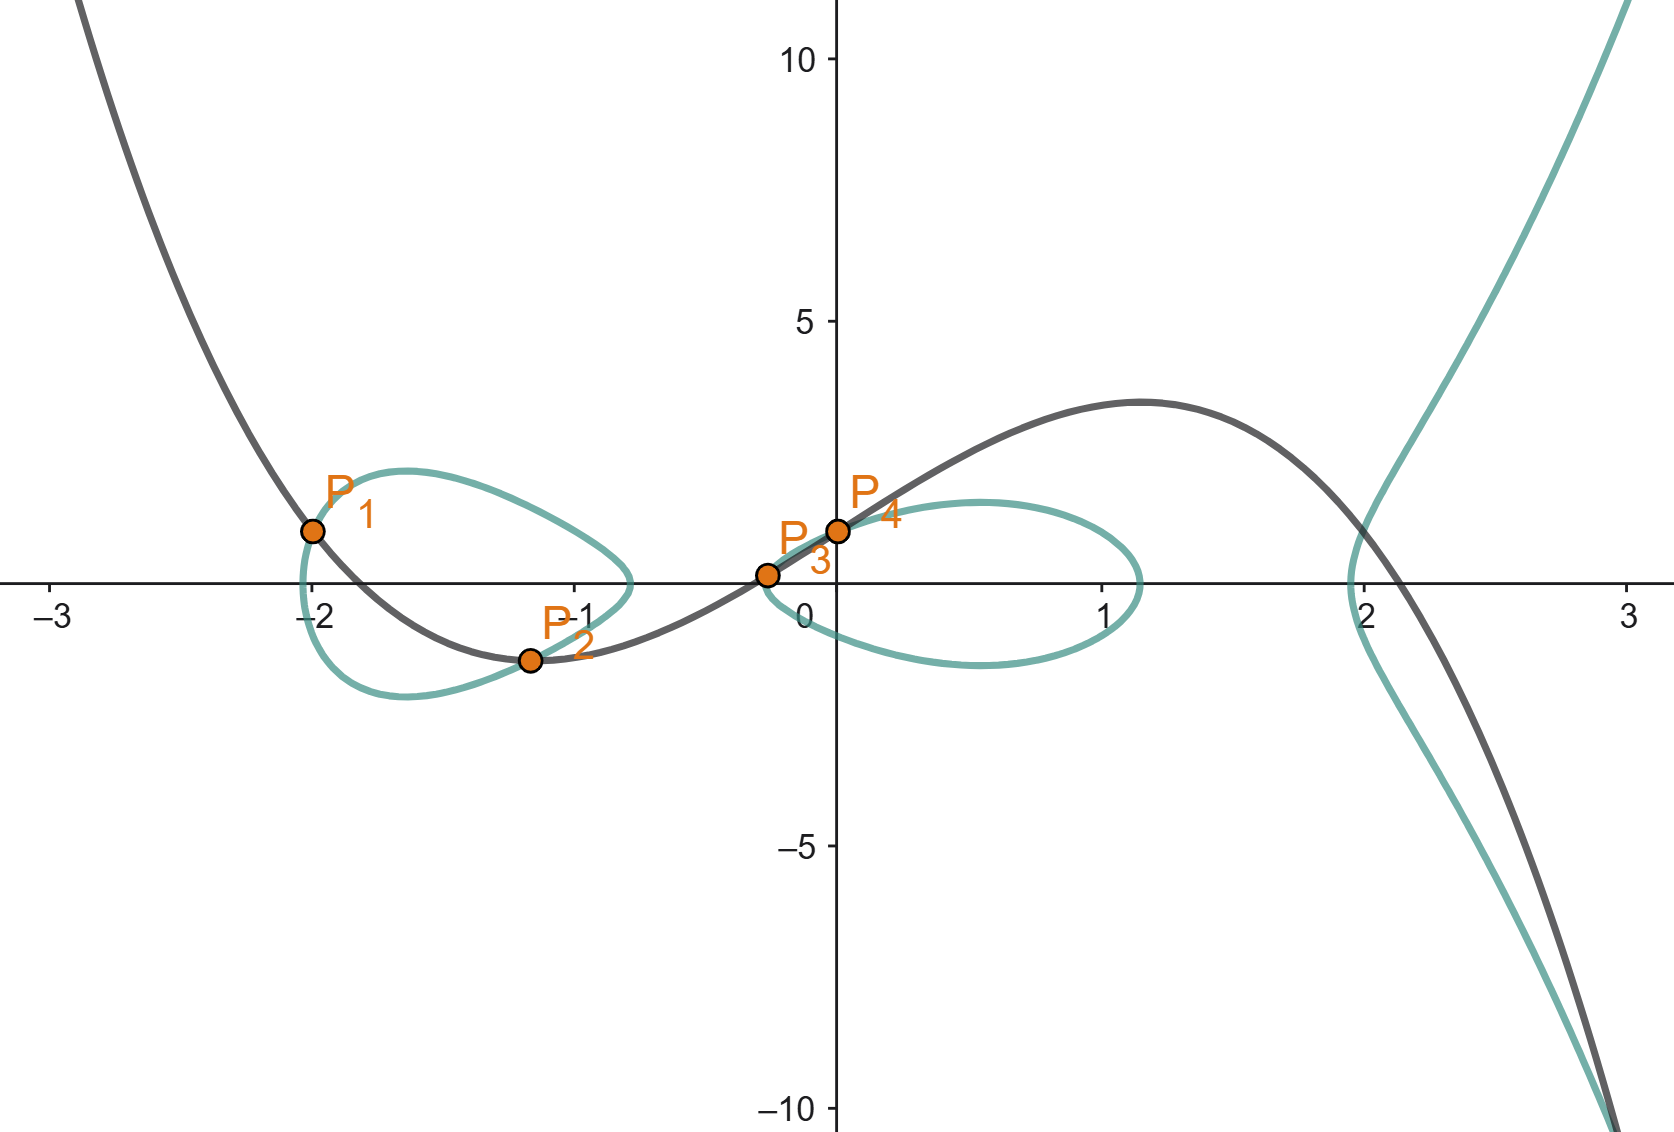
\includegraphics[width=0.4\textwidth]{images/div_add_2.png}
  \caption{Hyperelliptische Kurve mit $y^2=x^5-3x^3+4x+1$ über $\mathbb{R}$ Schnittpunkt mit $f$\\
    {\footnotesize Quelle: Eigene Darstellung mit GeoGebra}}
\end{figure}
Nun hat diese Funktion noch zwei weitere Schnittpunkte mit $C$ nämlich $Q_1=(2,0)$ und $Q_2=(3,-11)$. Durch alle Punkte kann der Hauptdivsior von $f$ beschrieben werden. $\operatorname{div}(f)=\sum_{i=1}^{4}(P_i)+(Q_1)+(Q_2)-6(\infty)$
\begin{figure}[htbp]
  \centering
  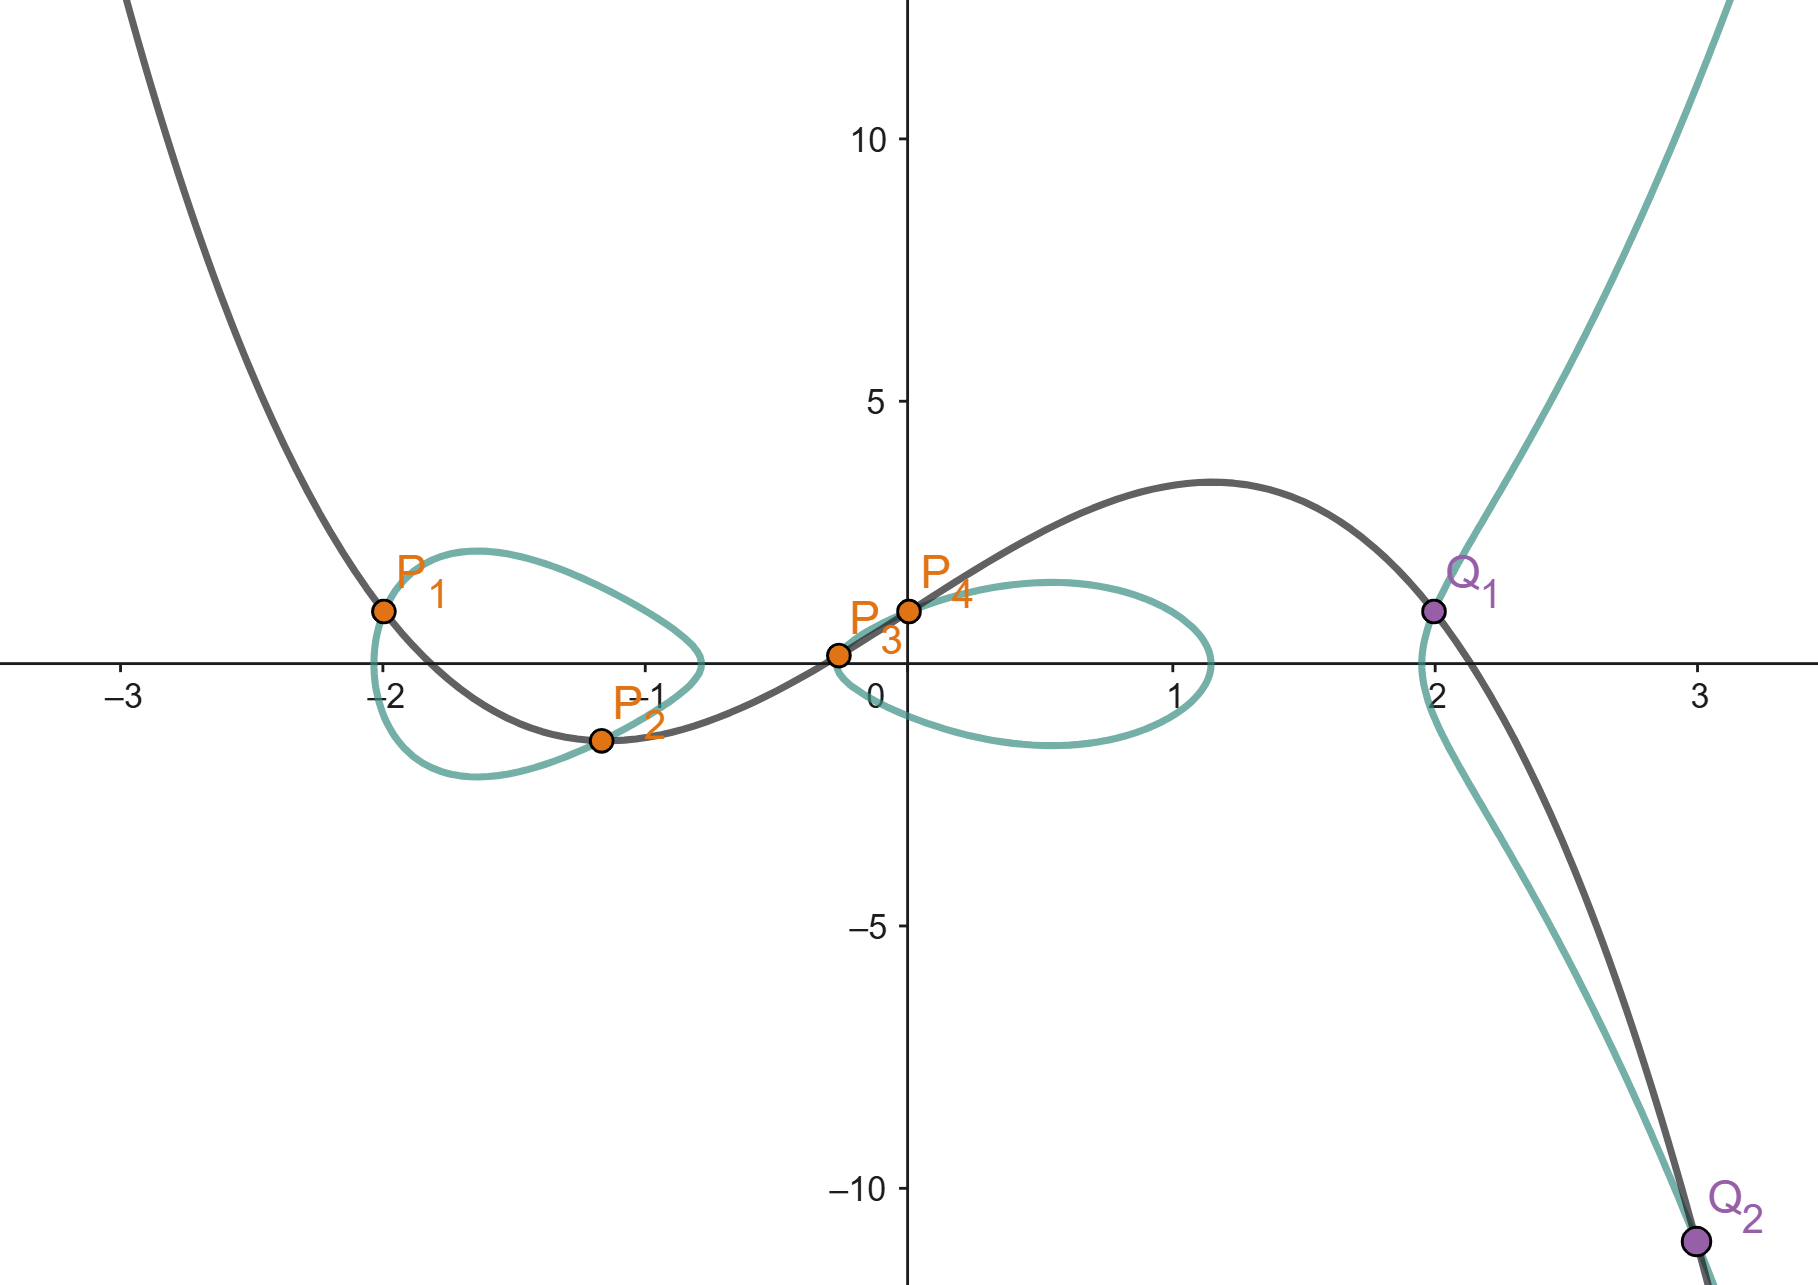
\includegraphics[width=0.4\textwidth]{images/div_add_3.png}
  \caption{Hyperelliptische Kurve mit $y^2=x^5-3x^3+4x+1$ über $\mathbb{R}$ Schnittpunkt mit $f$\\
    {\footnotesize Quelle: Eigene Darstellung mit GeoGebra}}
\end{figure}
Durch Spiegelung an der $x$-Achse wie bei den elliptischen Kurven erhält man dann den reduzierten Divisor mit $D\simeq (\overline{Q}_q)+(\overline{Q}_2)-2(\infty)$
\begin{figure}[htbp]
  \centering
  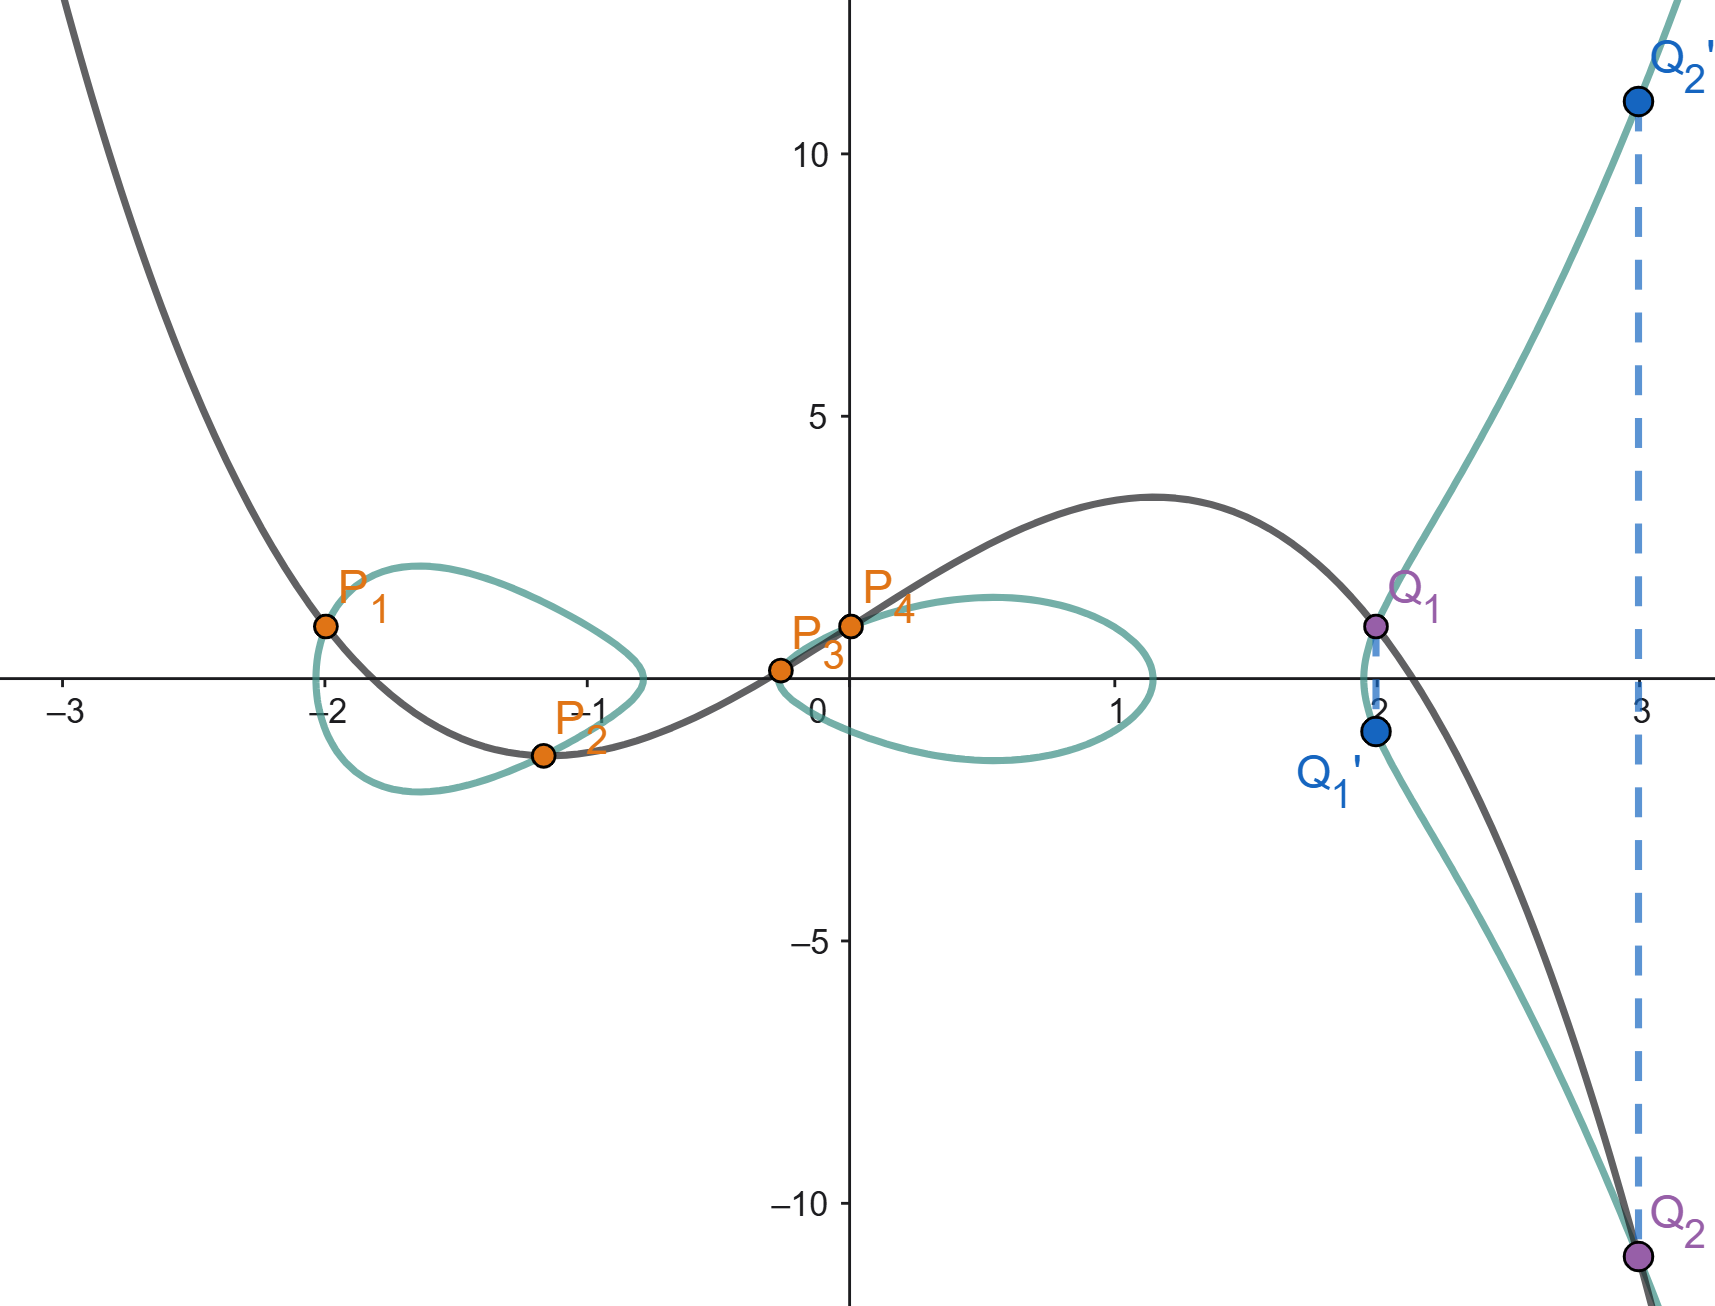
\includegraphics[width=0.4\textwidth]{images/div_add_4.png}
  \caption{Hyperelliptische Kurve mit $y^2=x^5-3x^3+4x+1$ über $\mathbb{R}$ Schnittpunkt mit $f$\\
    {\footnotesize Quelle: Eigene Darstellung mit GeoGebra}}
\end{figure}


Beispiel basiert von der Idee auf
\cite{scheidler15}









Hier noch Abbildung einfügen.




Sei $C$ eine Kurve dann können zwei Divisoren so aussehen.
\[
  D_1=2(P)-3(Q) \quad D_2 = 3(Q)+(R)-(S)
\]
\[
  D_1+D_2=2(P)+(R)-(S)
\]
Es kann auch Grad 0 erzeugt werden indem
\[
  \deg((P)+(Q)-2(\infty))=0
\]


\begin{definition}[Jacobische Varietät]
  Sei $C$ eine Kurve dann nennt man
  \[
    \operatorname{Jac}^0 C= Cl^0(C)=\{D\in \operatorname{Cl}(C)\mid \deg(D) = 0\}.
  \]
  die Jacobische Varietät von $C$ vom Grad $0$.
\end{definition}
Die Dimension $g$ von $\operatorname{Cl}^0(C)$ ist das Geschlecht der Kurve $C$. Über dem Grundkörper $\mathbb{C}$ ist dies identisch mit dem topologischen Gehsclehct, also die Anzahl der Löcher die $C$ in ihrer Riemannfläche hat.
\cite[S.78]{Cohen06} und \cite[S.149]{Hulek12}






\subsection{Der Verktorraum L(D)}

Sei $D$ ein Divisor auf $C$. Jeder Divisor wählt dann eine endliche Anzahl ein Punkten aus und ordnet ihm einen ganzahligen Wert zu. Es soll nun festegelgt werden wann es eine rationale Funktion mit Polen an den gewählten Punkten gibt und wann es Pole gibt die nicht schlechter als Ordnung $n_P$ bei $P$ sind.
Dabei ist $L(D)=\{f\in K\mid \operatorname{ord}_P(f)\geq -n_P \text{ für alle }P\in C\}$. Eine rationale Funktion $f$ gehört daher zu $L(D)$, wenn $\operatorname{div}(f)+D\geq 0$ oder wenn $f=0$ gilt. $L(D)$ ist dabei ein Vektorraum über $k$ und es gilt \(\dim(L(D))=l(D)\).


\begin{proposition}\label{prop:Gleichheit-zwei-Divisoren}
  Für zwei Divisoren $D$ und $D'$ gilt.
  \begin{enumerate}
    \item Wenn $D\leq D'$, dann gilt $L(D)\subset L(D')$ und damit \(\dim_k(L(D')/L(D))\).
    \item Wenn $D\equiv D'$, dann ist $\deg(D)=\deg(D')$.
  \end{enumerate}
\end{proposition}
\begin{proof}
  Beweis in \cite[S.98]{Fuelton08} (1)+(3)
\end{proof}
Sei $D\in\operatorname{Div}_C$. Dann ist
\[
  L(D)=\{f\in K(C)\mid \div(f)\geq -D\}
\]
und $l(D)=\dim_K(L(D))$.
\begin{proposition}\label{prop:l(d)-endlich}
  Seien $D$ und $D'$ Divisoren.
  \begin{enumerate}
    \item Wenn $D\leq D'$, dann gilt $L(D)\subset L(D')$ und damit
          \[
            \dim_k(L(D')/L(D))\leq \deg(D'-D).
          \]
    \item Wenn $\deg(D)<0$, dann ist $L(0)=k$ und $L(D)=0$
    \item wenn $D\equiv D'$ gilt, dann folgt $l(D)=l(D')$.
  \end{enumerate}
\end{proposition}
\begin{proof}
  \begin{enumerate}
    \item Es ist $D'=D+P_1+\dots P_s$, wobei $P_i$ Punkte auf der Kurve $C$ sind, mit $s=\deg(D'-D)$. Außerdem ist $L(D)\subset L(D+P_1)\subset\dots\subset \dim(L(D+P_1+\dots P_s))$ und daher ist es aureichend zu zeigen, dass $(L(D+P)/L(D))\leq 1$
          Für drei Vektorräume $U\subset W \subset V$ mit $V/U$ endlich dimensional gilt mit der Dimensionalformel für einen Quotientenvektorraum (vgl.~\cite[S.~69]{Bosch06}), dass
          \[
            \dim(V/U)=\dim(V)-\dim(U),\quad \dim(V/W)=\dim(V)-\dim(W),\quad \dim(W/U)=\dim(W)-\dim(U).
          \]
          Damit folgt
          \begin{align*}
            \dim (V/W) + \dim (W/U) & = \dim(V)-\dim(W) + \dim(W)-\dim(U) \\
                                    & = \dim(V)-\dim(U)
                                    & = \dim(V/U).
          \end{align*}
          Daher muss gezeigt werden $l(D')-l(D)\leq s\Longleftrightarrow \dim(L(D')/L(D))\leq \deg(D'-D)$.

          Sei nun $P\in C$ und $r=n_P$ der Koeffizient von $P$ im Divisor $D$. Sei $t$ ein Parameter des Rings der algebraischen Varietäten $\mathcal{O}_P(C)$ mit $\operatorname{ord}_P(t)=1$.

          Wenn $f\in L(D)$ gilt, dann gilt nach Definition von $L(D)$, dass $f=t^{-r}(a_0+a_1t+a_2t^2+\dots)$ und  $\operatorname{ord}_P(f)\geq -r$ ist. Wenn nun $f\in L(D+P)$ liegt,dann ist $f=t^{-(r+1)}(a_0+a_1t+a_2t^2+\dots)$ dann muss \(\operatorname{ord}_P(f)\geq -r-1\) gelten. Es wird nun die Abbildung $\phi:L(D+P)\rightarrow k, f\mapsto(t^{r+1}f)(P)$ definiert.

          Da $\operatorname{ord}_P(t)=1$ gilt, folgt für jedes $f\in L(D+P)$, dass $\operatorname{ord}_P(t^{r+1}f)=r+1+\operatorname{ord}_P(f) \geq 0$. Dahert ist $t^{r+1}f$ am Punkt $P$ regulär und daraus folgt $\phi$ ist wohldefiniert.

          Für $f\in L(D)$ gilt \(\operatorname{ord}_P(t^{r+1}f)\geq 1\) und daher verschwindet $t^{r+1}f$ am Punkt $P$, sodass $\phi(f)=0$ gilt.

          Für $f\in L(D+P)$ folgt mit $\phi(f)=0$, dass $\operatorname{ord}_P(t^{r+1}f)\geq1$ und damit
          \[
            \operatorname{ord}_P(f)\geq -r.
          \]
          Damit folgt $f\in L(D)$. Es ist dann $\ker(\phi)=L(D)$, also der Koeffizient des höchstens zugelassenen Polterms.


          $\phi$ ist somit ist eine lineare Abbildung mit $\ker(\phi)=L(D)$. Es kann dann $\overline{\phi}:L(D+P)/L(D)\rightarrow k$ definiert werden.
          \textbf{Später noch fertig machen}
    \item Sei $D\equiv D'$ was gleichbedeutend ist mit $D'=D+\operatorname{div}(z)$ für ein $z\in K$. Sei nun $\psi:L(D)\rightarrow L(D'), f\mapsto \frac{f}{z}$. Es gilt dann
          \begin{align*}
            \operatorname{div}(\frac{f}{z})+D' & =\operatorname{div}(f)-\operatorname{div}(z)+D+\operatorname{div}(z) \\
                                               & = \operatorname{div}(f)+D
                                               & \geq 0.
          \end{align*}
          Damit ist $\frac{f}{z}\in L(D')$ und $\psi$ wohldefiniert. $\psi$ ist offensichtlich eine lineare bijektive Abbildung mit $\psi^{-1}:L(D')\rightarrow L(D), f \mapsto fz$. Daraus folgt, dass $psi$ ein Isomorphismus zwischen den Vektorräumen ist, also$L(D)\simeq L(D')$. Daraus folgt $l(D)\dim(L(D))=\dim(L(D'))=l(D')$.
  \end{enumerate}
  Beweis in \cite[S.99]{Fuelton08}
\end{proof}

\begin{proposition}\label{prop:divisor-tau}
  Sei $x\in K, x\notin k$. Dann ist $Z=(x)_0$ der Divisor von Nullen von $x$. Sei nun zusätzlich $n=[K:k(x)]$, dann gilt
  \begin{enumerate}
    \item $Z$ ist ein positiver Divisor vom Grad $n$.
    \item Es gibt eine Konstante $\tau$, sodass \(l(rZ)\geq rn-\tau\) für alle $r$ gilt.
  \end{enumerate}
\end{proposition}
\begin{proof}
  Beweis in \cite[S.100]{Fuelton08}(2)
\end{proof}

\begin{theorem}[Riemmann-Roch]
  Sei $C$ eine irreducible Kurve über $K$. Dann exestiert eine Ganzzahl $g\geq 0$, sodass für jeden Divisor $D\in\operatorname{Div}_C$ gilt
  \[
    l(D)\geq\deg(D)+1-g.
  \]
  Für alle $D\in\operatorname{Div}_C$ mit $\deg(D)>2g-2$ gilt sogar Gleichheit $l(D)=\deg(D)-g+1$.
\end{theorem}
\cite[S.66]{Cohen06}
\cite[S.68]{Cohen06}
\cite[S.160]{Hulek12}

\begin{proof}
  Sei $K=k(C)$ der Funktionenkörper der Kurve $C$ über dem algebraisch abgeschlossenen Körper $k$. Sei $D$ ein Divisor, dann wird für den Beweis $s$ definert als
  \[
    s(D)=\deg(D)+1-l(D).
  \]
  Es soll nun ein $g$ gefunden werden, sodass $s(D)\leq g$ für alle Divisoren $D$ gilt.

  Es gilt mit Proposition~\ref{prop:l(d)-endlich}~(2), dass $l(0)=\dim_k L(0)=1$ und damit
  \[
    s(0)=\deg(0)+1-l(0)=0+1-1=0.
  \]
  Daher muss jedes $g$ die Ungleichung $g\geq 0$ erfüllen. Seien nun $D$ und $D'$ zwei Divisoren mit $D\equiv D'$. Nach Porposition~\ref{prop:Gleichheit-zwei-Divisoren} gilt $\deg(D)=\deg(D')$ für $D'\equiv D$. Zusätzlich folgt aus Proposition~\ref{prop:l(d)-endlich}, dass $l(D)=l(D')$ gilt. Mit beiden Propositionen erhält man
  \[
    s(D')=\deg(D')+1-l(D')=\deg(D)+1-l(D)=s(D).
  \]
  Seien nun $D,D'\in\operatorname{Div}(C)$ mit $D\leq D'$. Dann gilt $L(D)\subset L(D')$ und mit Proposition~\ref{prop:Gleichheit-zwei-Divisoren} (1) folgt dann
  \[
    \dim_k(L(D')/L(D))\leq\deg(D'-D).
  \]
  Mit der Dimensionsformel für Quotientenvektorräume (vgl. Bosch~\cite[S.69]{Bosch06}) folgt
  \( \dim_k(L(D')/L(D)) = \dim_k(L(D')) - \dim_k(L(D)) = l(D') - l(D)\) und damit für die Ungleichung
  \[
    l(D')-l(d)\leq \deg(D'-D).
  \]
  Da die Gradabbildung ein Gruppenhomorphismus ist, ergibt sich
  \begin{align*}
    l(D')-l(D)     & \leq \deg(D'-D)       \\
    \deg(D)+1-l(D) & \leq \deg(D')+1-l(D') \\
    s(D)           & \leq s(D').
  \end{align*}
  Sei $x\in K,x\notin k$ und $Z=(x)_0$  Nullstellendivisor von $x$. Außerdem sei $n=[K:k(x)]=\deg(Z)$. Nach Proposition~\ref{prop:divisor-tau} exestiert eine kleinste Zahl $\tau$, sodass \(rn-\tau\leq l(rZ)\) für alle $r\geq 0$ gilt. Daraus folgt
  \begin{align*}
    s(rZ) & = \deg(rZ)+1-l(rZ)  \\
          & = r\deg(Z)+1-l(rZ)  \\
          & = rn+1-l(rZ)        \\
          & \leq rn+1-(rn-\tau) \\
          & = \tau + 1
  \end{align*}
  Nach Proposition~\ref{prop:divisor-tau}~(1) ist $Z$ ein positiver Divisor. Somit gilt für alle $\in\mathbb{N}_{>0}$, dass $rZ\leq(r+1)Z$. Mit der zuvor gezeigten Monotonie folgt dann \(s(rZ)\leq s((r+1)Z)\). Die Folge ist also monoton wachsen, ganzzahlig und nach oben durch $\tau+1$ beschränkt. Aufgrund der Minimalität von $\tau$ muss sogar gelten $s(rZ)=\tau+1$ für alle hinreichend großen $r>0$. Es wird nun $g=\tau+1$ gesetzt.

  Es bleibt zu zeigen, dass $s(D)\leq g$ für jeden Divisor $D$ gilt. Dazu wird ein Divisor $D'\equiv D$ gesucht für den $D'\leq rZ$ für $r\geq 0 $ gilt. Sei nun $Z=\sum_{P\in C}n_P P$ wie oben definiert und $D=\sum_{P\in C}m_P P$. Sei $f$ eine rationale Funktion, dann gilt $D'= D - \operatorname{div}(f)$. Damit ist dann $D\equiv D$ und
  \[
    D'= \sum_{P\in C}(m_P P)-\sum_{P\in C}\operatorname{ord}_P(f)P=\sum_{P\in C}(m_P -\operatorname{ord}_P(f))P.
  \]
  Es soll also $(m_P -\operatorname{ord}_P(f))\leq rn_P$ gelten.

  Setze nun $y=x^{-1}$ und $T=\{P\in X\mid m_p>0\text{ und }\operatorname{ord}_P(y)\geq 0\}$. Es soll eine Funktion konstruiert werden, die an jedem Punkt $P\in T$ mindestens mit
  der Ordnung $m_P$ verschwindet. Sei dazu \(f=\prod_{P\in T}(y-y(P))^{m_P}\). Für den ersten Fall ist $\operatorname{ord}_P(y)\geq 0$. Ist $P\in T$, so gilt $(y-y(P))(P)=y(P)-y(P)=0$ und damit $\operatorname{ord}_P(y-y(P))\geq 1$. Daraus folgt
  \[
    \operatorname{ord}_P((y-y(P))^{m_P})=m_P\operatorname{ord}_P(y-y(P))\geq m_P
  \]
  Da $y$ im Punkt $P$ regulär ist, sind auch die übrigen Faktoren von $f$ im Punkt $P$ regulär. Damit folgt dann
  \begin{align*}
    m_P                          & \leq \operatorname{ord}_P(f) \\
    m_P -\operatorname{ord}_P(f) & \leq 0.
  \end{align*}
  Ist dagegen $P\notin T$ mit $\operatorname{ord}_P(y)\geq0$ folgt nach Vorraussetzung $m_P\leq0$. Da $f$ auch an diesem Punkt regulär ist, gilt $\operatorname{ord}_P(f)\geq0$. Somit folgt auch hier
  \[
    m_P-\operatorname{ord}_P(f)\leq0.
  \]
  Für den zweiten Fall sei $\operatorname{ord}_P(y)<0$, so folgt wegen $y=x^{-1}$, dass
  \[
    \operatorname{ord}_P(x)
    =-\operatorname{ord}_P(y)>0.
  \]
  Damit ist $P$ eine Nullstelle von $x$, sodass $n_P>0$ gilt. Für ein hinreichend großes $r\geq 0$ gilt dann \(m_P-\operatorname{ord}_P(f)\leq rn_P\). Damit folgt gesamt
  \[
    D'=D-\operatorname{div}(f)\leq rZ.
  \]

  Mit den bereits gezeigten Aussagen ergibt sich dann
  \[
    s(D)=s(D')\leq s(rZ)\leq g.
  \]
  und daher nach Definition von $s$
  \begin{align*}
    \deg(D)+1-l(D) & \leq g            \\
    l(D)           & \geq \deg(D)+1-g.
  \end{align*}
  Da für hinreichend große $r$ bereits $s(rZ)=g$ gilt, ist $g$ die kleinste ganze Zahl, für die diese Ungleichung für alle Divisoren erfüllt ist.
\end{proof}
Beweis nach \cite[S.101--102]{Fuelton08}



Für ein Geschlecht größer 1, ist es nun nicht mehr möglich die abelsche Gruppe mit Hilfe der Punkte auf einer elliptischen Kurve $E$ und dem Punkt im Unendlichen zu bilden. Es wird daher eine endliche Summe von Punkte aus Gruppen Elementen genutzt, wobei diese koeffizientenweise addiert werden $(P+Q)\oplus(R+Q)=P +2Q+R$. Dies führt aber in einer endlichen Gruppe zu immer länger werdenen Darstellung der Gruppenelemente. Daher wird die Quotientengruppe dieser Gruppe mit allen Puntke die auf einer Funktion leigen genutzt.

Wenn die Charakteristik von $K$ ungleich $2$ ist, kann man das Quadrat auf der linken Seite vollenden und es in die Form
\[
  C:y^2=f(x)
\]
bringen, wobei $f$ normiert ist und vom Grad $2g+1$. Aus der Nichtsingularität folgt $2y=0=f'(x)$ darf kein Punkt auf der Kurve erfüllen. Da $y=0$ und damit $f(x)=0$ gilt, ist das äquivlanz zu sagen, dass kein $x$ $f(x)=0=f'(x)$ erfüllt. Also $f(x)$ darf keine mehrfachen Nullsten haben
\subsection{Gruppenstruktur auf elliptischen Kurven}
\cite[S.304--305]{Cohen06},


Bild einer Hyperelliptischen Kurve einfügen


Durch das Bild wird klar, dass es nicht mehr möglich ist die geometrische Methode mit der Gerade/Tangente und Spiegelung des Schnittpunktes wie bei elliptischen Kurven nutzen kann.

Um eine Gruppe zu bilden

\begin{definition}[Divisorklassengruppe]
  Sei $C$ eine hyperelliptische Kurve mit Geschlecht $g$ über $K$. Die Divisorklassengruppe von $C$ mit Grad $0$ ist gegeben durch
  \[
    \operatorname{Div}^0_C=\left\{D=\sum_{P\in C}n_P P\mid n_P\in\mathbb{Z},n_P=0 \text{ für fast alle }P\in C, \sum_{P\in C}n_P=0 \text{ mit }\sigma(D)=D \text{ für alle }\sigma\in G_K\right\}
  \]
  Das bedeutet, dass der Divisior über $K$ definiert ist. Das ist äquivalent zu $n_{\sigma(P)}=n_P$ für alle $\sigma\in G_K$, die Galois Gruppe von $K$.
\end{definition}

\begin{definition}
  Die Divisorklassengruppe $\operatorname{Pic}_C^0$ von $C$ ist die Quotientengruppe von $\operatorname{Div}_C^0$ mit der Gruppe der Pinzipiellen Divisoren, das sind die Divisoren, welche Ordnung $0$ haben und aus Funktionen entstehen.
  Jede Divisiorklasse kann durch eine endliche Summe dargestellt werden
  \[
    \sum_{i=1}^r P_i-rP_\infty, P_i\in C\setminus\{P_\infty\}, r\leq g
  \]
  mit $P_i=(x_i,y_i)\neq (x_j,-y_j-h(x_j))=-P_j$ für $i\neq j$
\end{definition}
Anmerkung $\infty$ muss eventuell zu $\mathcal{O}$ geändert werden

Die nachfolgende Repräsentation ist vor allem für Implementation nützlicher. Hier kann man direkt den Körper der Definition von Gruppenelementen ablesen. Das ist möglich, weil die Divisorklassengruppe isomorph ist zu der Idealklassengruppe vom Funktionenfeld $K(C)$ ist. Außerdem ist die Divisiorklassengruppe isomorph zu der Gruppe der $K$-rationalen Punkte auf dem Jacobian $J_C$ für $C$. Die Mumforddarstellung druckt diese Isomorphie aus. Die Quotientengruppe $J=D^0/P$ nennt man dann das Jacobian der Kurve $C$.
Es werden nun die Gruppenelemente Divisorklassen genannt.

\begin{definition}[Mumforddarstellung]
  Sei $C$ eine hyperelliptische Kurve vom Geschlecht $g$ mit der Gleichung $C:y^2+h(x)y=f(x)$ mit $h,f\in K[X]$, $\deg(f)=2g+1$ und $\deg(h)\leq g$. Jede nichtriviale Divisiorklasse über $K$ kann dargestellt werden als ein einzigartiges Paar von Polynomen $u(x)$ und $v(x)$ mit $u,v\in K[x]$, wenn gilt
  \begin{enumerate}
    \item $u$ ist nomiert,
    \item $\deg v< \deg u\leq g$,
    \item $u\mid v^2+vh-f$.
  \end{enumerate}
\end{definition}

Sei $D=\sum_{i=1}^r P_i-rP_\infty$ mit $P_i\neq P_\infty$, $P_i\neq P_j$ für $i\neq j$ und $r\leq g$. Sei $P_i=(x_i,y_i)$, dann wird die Divisorklasse von $D$ durch
\[
  u(x)=\prod_{i=1}^r(x-x_i)
\]
repräsentiert. Wenn $P_i$ $n_i$-mal auftaucht, dann
\[
  \left(\frac{d}{dx}\right)^j [v(x)^2+v(x)h(x)-f(x)]_{x=x_i}=0, \quad \text{für } 0\leq j\leq n_i-1.
\]



Nächste Punkte
\begin{enumerate}
  \item Lineare Äquivalenzen und Divisiorklasse (Hauptdivisioren und Quotientengruppen)
  \item Jacobische Varietäten
  \item Reduzierte Divisoren und Mumford-Darstellung
  \item Cantors Algorithmus
  \item Hyperellitpisches DL-Problem
\end{enumerate}
\section{First Real Chapter addressing first Research Problem}\label{sec:problem1}
%%% ===============================================================================

\emph{Purpose and scope}.
After you stated research context (SM1), research problem (SM2), and research method (SM3) in \zcref{sec:introduction}, the remainder of your entire report addresses execution (SM4), results (SM5), and interpretation (SM6).
You usually do this by addressing various sub-problems again through scientific arguments following the 6 steps SM1-SM6.

Have a short chapter introduction that recalls and explains the first research problem of your thesis.
The problem has to show up in the introduction in \zcref{sec:introduction:research-question} already.
This provides the background (SM1) for this chapter while the first research problem of the thesis becomes the research question/hypothesis (SM2) for this chapter.

Next, explain in the chapter intro how you solve the research problem in this chapter by breaking it down in further sub-problems.
By this, you outline the method (SM3) through which you are going to solve the problem of this chapter.
This is necessary to give the reader guidance of what's to come in this chapter and how it fits into the thesis as a whole.
Explain that you will address the first sub-problem in \zcref{sec:problem1:subproblem1} and the second sub-problem in \zcref{sec:problem1:subproblem2}, etc. The sections then provide the details for execution and results.

% ---------------------------------------------------------------------------------
\section{First Sub-Problem}\label{sec:problem1:subproblem1}
% ---------------------------------------------------------------------------------

\emph{The first paragraph describes the first sub-problem and develops the requirements a solution has to satisfy (SM2 for this section).}
The requirements have to be based on the knowledge and reasoning developing in the preceding chapters and sections.
Try to use an example to illustrate the problem and the desired properties of the solution.
Check that every term/concept you use here has already been defined already in a previous section.
If you cannot describe your problem without defining new terms, you may have to add another section before this one that develops the terms and concepts you need to explain the problem.

\emph{The second paragraph describes the method/approach how you address the problem (SM3 for this section).}
Describe the method in a level of detail that allows another student to reproduce your steps.
Make use of appendices % (see \zcref{sec:appendix1})
if certain details take too much space.

\emph{The third, fourth, and following paragraph provides details on applying the method or developing a new approach, i.e., execution (SM4) and may explain results (SM5)}, i.e. details on the steps needed to reproduce the results.

Results (SM5) can come in many forms, e.g., conceptual diagrams, algorithms, tables, charts, a list of articles from a literature research etc. You must reference them (``\zcref{fig:my_label} shows.
..'') and describe the results in text.
If you use diagrams, tables, or charts, you cannot expect the reader to know what to you expect them to see in a diagram, table or chart.
Describe to them how to read these, explain the meaning of particular elements, point out special observations.
Describe the results, but do not interpret them.
Make use of appendices if certain details take too much space.

\begin{figure}
  \centering
  %%%\includegraphics{/path/to/figure.pdf}
  \caption{A scientific figure that has to be explained in the text}
  \label{fig:my_label}
\end{figure}

\emph{After describing the results, you may interpret them (SM6).}
Here you can infer what a particular observation means (for you), how it can be applied, or what others can do with it.
Do not interpret your results before you have described all of them.
This is a common mistake done by most beginner writers.
You want to quickly get to the point, which is the final finding or interpretation.
But you forget that your reader does not understand yet what you are interpreting - they do not know yet what you do know.
Interpret the results only after describing all of them.
The interpretation must be based on the written description only.
Then you can be sure that your readers can follow your interpretation and reach the same conclusions as you have.

Ideally, your interpretation leads to the next sub-problem in \zcref{sec:problem1:subproblem2}.

% ---------------------------------------------------------------------------------
\section{Second Sub-Problem}\label{sec:problem1:subproblem2}
% ---------------------------------------------------------------------------------

You now build on the solution to the first sub-problem of \zcref{sec:problem1:subproblem1} (SM1) and recall second sub-problem (SM2, you detailed in the introduction of this chapter) and follow the same pattern as before (SM3-SM6).

Note that not all sections may not include all parts SM1-SM6 in all detail.
Some sections need not restate the background (SM1) or the research problem (SM2) if a previous section already defined them.
Sometimes, a section is only dedicated to describing the method (SM3) and execution (SM4) and does not contain any results or interpretations.
Sometimes results (SM5) and interpretations (SM6) only come in the evaluation chapter.

What is important for you when you are writing a scientific argument is not to slavishly have SM1-SM6 in each section explicitly, but that you are always fully aware of the following:
%
\begin{itemize}
  \item Which step of a scientific argument am I currently writing (SM1, SM2, ..., SM6)?
  \item Does the step that I am writing come in the right order, i.e., if you are writing about execution (SM4, e.g., details of building a model), is there a preceding paragraph or section that describes the method (SM3) and is that one preceded by a clear statement of the (sub-)problem addressed (SM2)?
  \item Are you really \emph{not} writing interpretation SM6 before SM5, SM4, or SM3?
  \item Is it clear to the reader which part of the scientific argument you are currently making?
\end{itemize}




\section{Kryptographie auf Hyperelliptischen Kurven}

RSA lange Schlüssellange und aufwendige Berechnungen, daher ungeeignet für kleine Geräte, HCC liefert eine leichtgewichtigerte Variante. HCC behebt Passwörter, Integerfaktorisierung und die Verschlüsselung des öffentlichen Schlüssels (soll mehr Sicherheit liefern als ECC).

\cite[59--60]{Salam21}


\textbf{Nur Kurzzusammenfassung}

Kurve vom Geschlecht $g=2$. Gruppe ist $J_C(\mathbb{F}_q)$. Gruppenelement ist Divisorklasse (anstatt Kurvenpunkt wie bei ECC). Addition von Divisorkalssen. DL-Problem ist $\mathcal{Q}=k\mathcal{P}$ mit $\mathcal{P},\mathcal{Q}\in J_C(\mathbb{F_q})$.

Ein Element im Jacobischen kann bei Geschlecht zwei durch reduzierten Divisor dargestellt werden $D=P+Q-2\infty$. Die Mumford-Darstellung speichert den Divisor mit zwei Polynomen $(u(c),v(x))$.

Beispiel: $C:y^2=x^5+x+1$ über $\mathbb{F}_{11}$ und $g=2$. $P=(0,1)$ und $Q=(1,5)$ dann ergibt sich $u(x)=x(x-1)=x^2-x$ und $v(x)=4x+1$. Damit repräsentiert $(x^2-x,4x+1)$ die Divisorklasse $[P+Q-2\infty]$.

Addition: \([D_1]+[D_2]=[D_1+D_2]\). Neuer Divisor kann mehr als $g$ Punkte im positiven endlichen Anteil enthalten. Mit Canotr-Algorithmus reduziert, dadurch enthält man wieder einen eindeutig bestimmten reduzierten Divisor durch ein Mumford-Paar mit $\deg u\leq g$ dargestellt.

